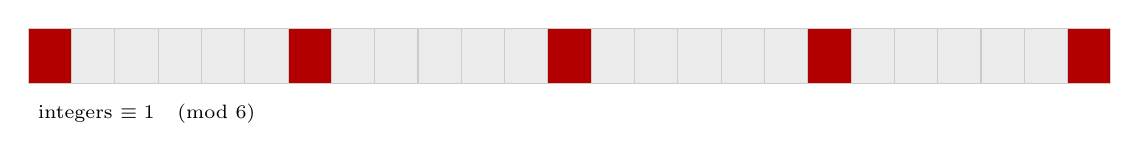
\begin{tikzpicture}[x=0.55cm,y=0.7cm]
\foreach \n/\hit in {1/1,2/0,3/0,4/0,5/0,6/0,7/1,8/0,9/0,10/0,11/0,12/0,13/1,14/0,15/0,16/0,17/0,18/0,19/1,20/0,21/0,22/0,23/0,24/0,25/1}{
  \ifnum\hit=1
    \fill[red!70!black] ({\n-1},0) rectangle (\n,1);
  \else
    \fill[black!8] ({\n-1},0) rectangle (\n,1);
  \fi
  \draw[black!20] ({\n-1},0) rectangle (\n,1);
}
\node[font=\scriptsize,anchor=west] at (0,-0.55) {integers $\equiv 1\pmod 6$};
\end{tikzpicture}
